\begin{figure}
    \centering
    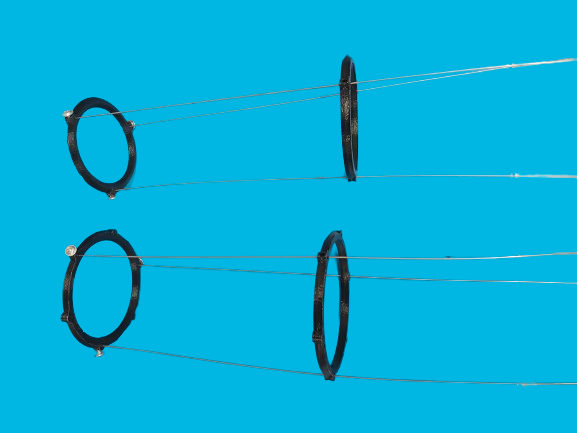
\includegraphics[width=0.6\textwidth]{arm-segments}
    \caption{Arm segments}
    \label{arm-segmentes}
\end{figure}


\begin{figure}
    \centering
    \begin{subfigure}[b]{0.3\textwidth}
        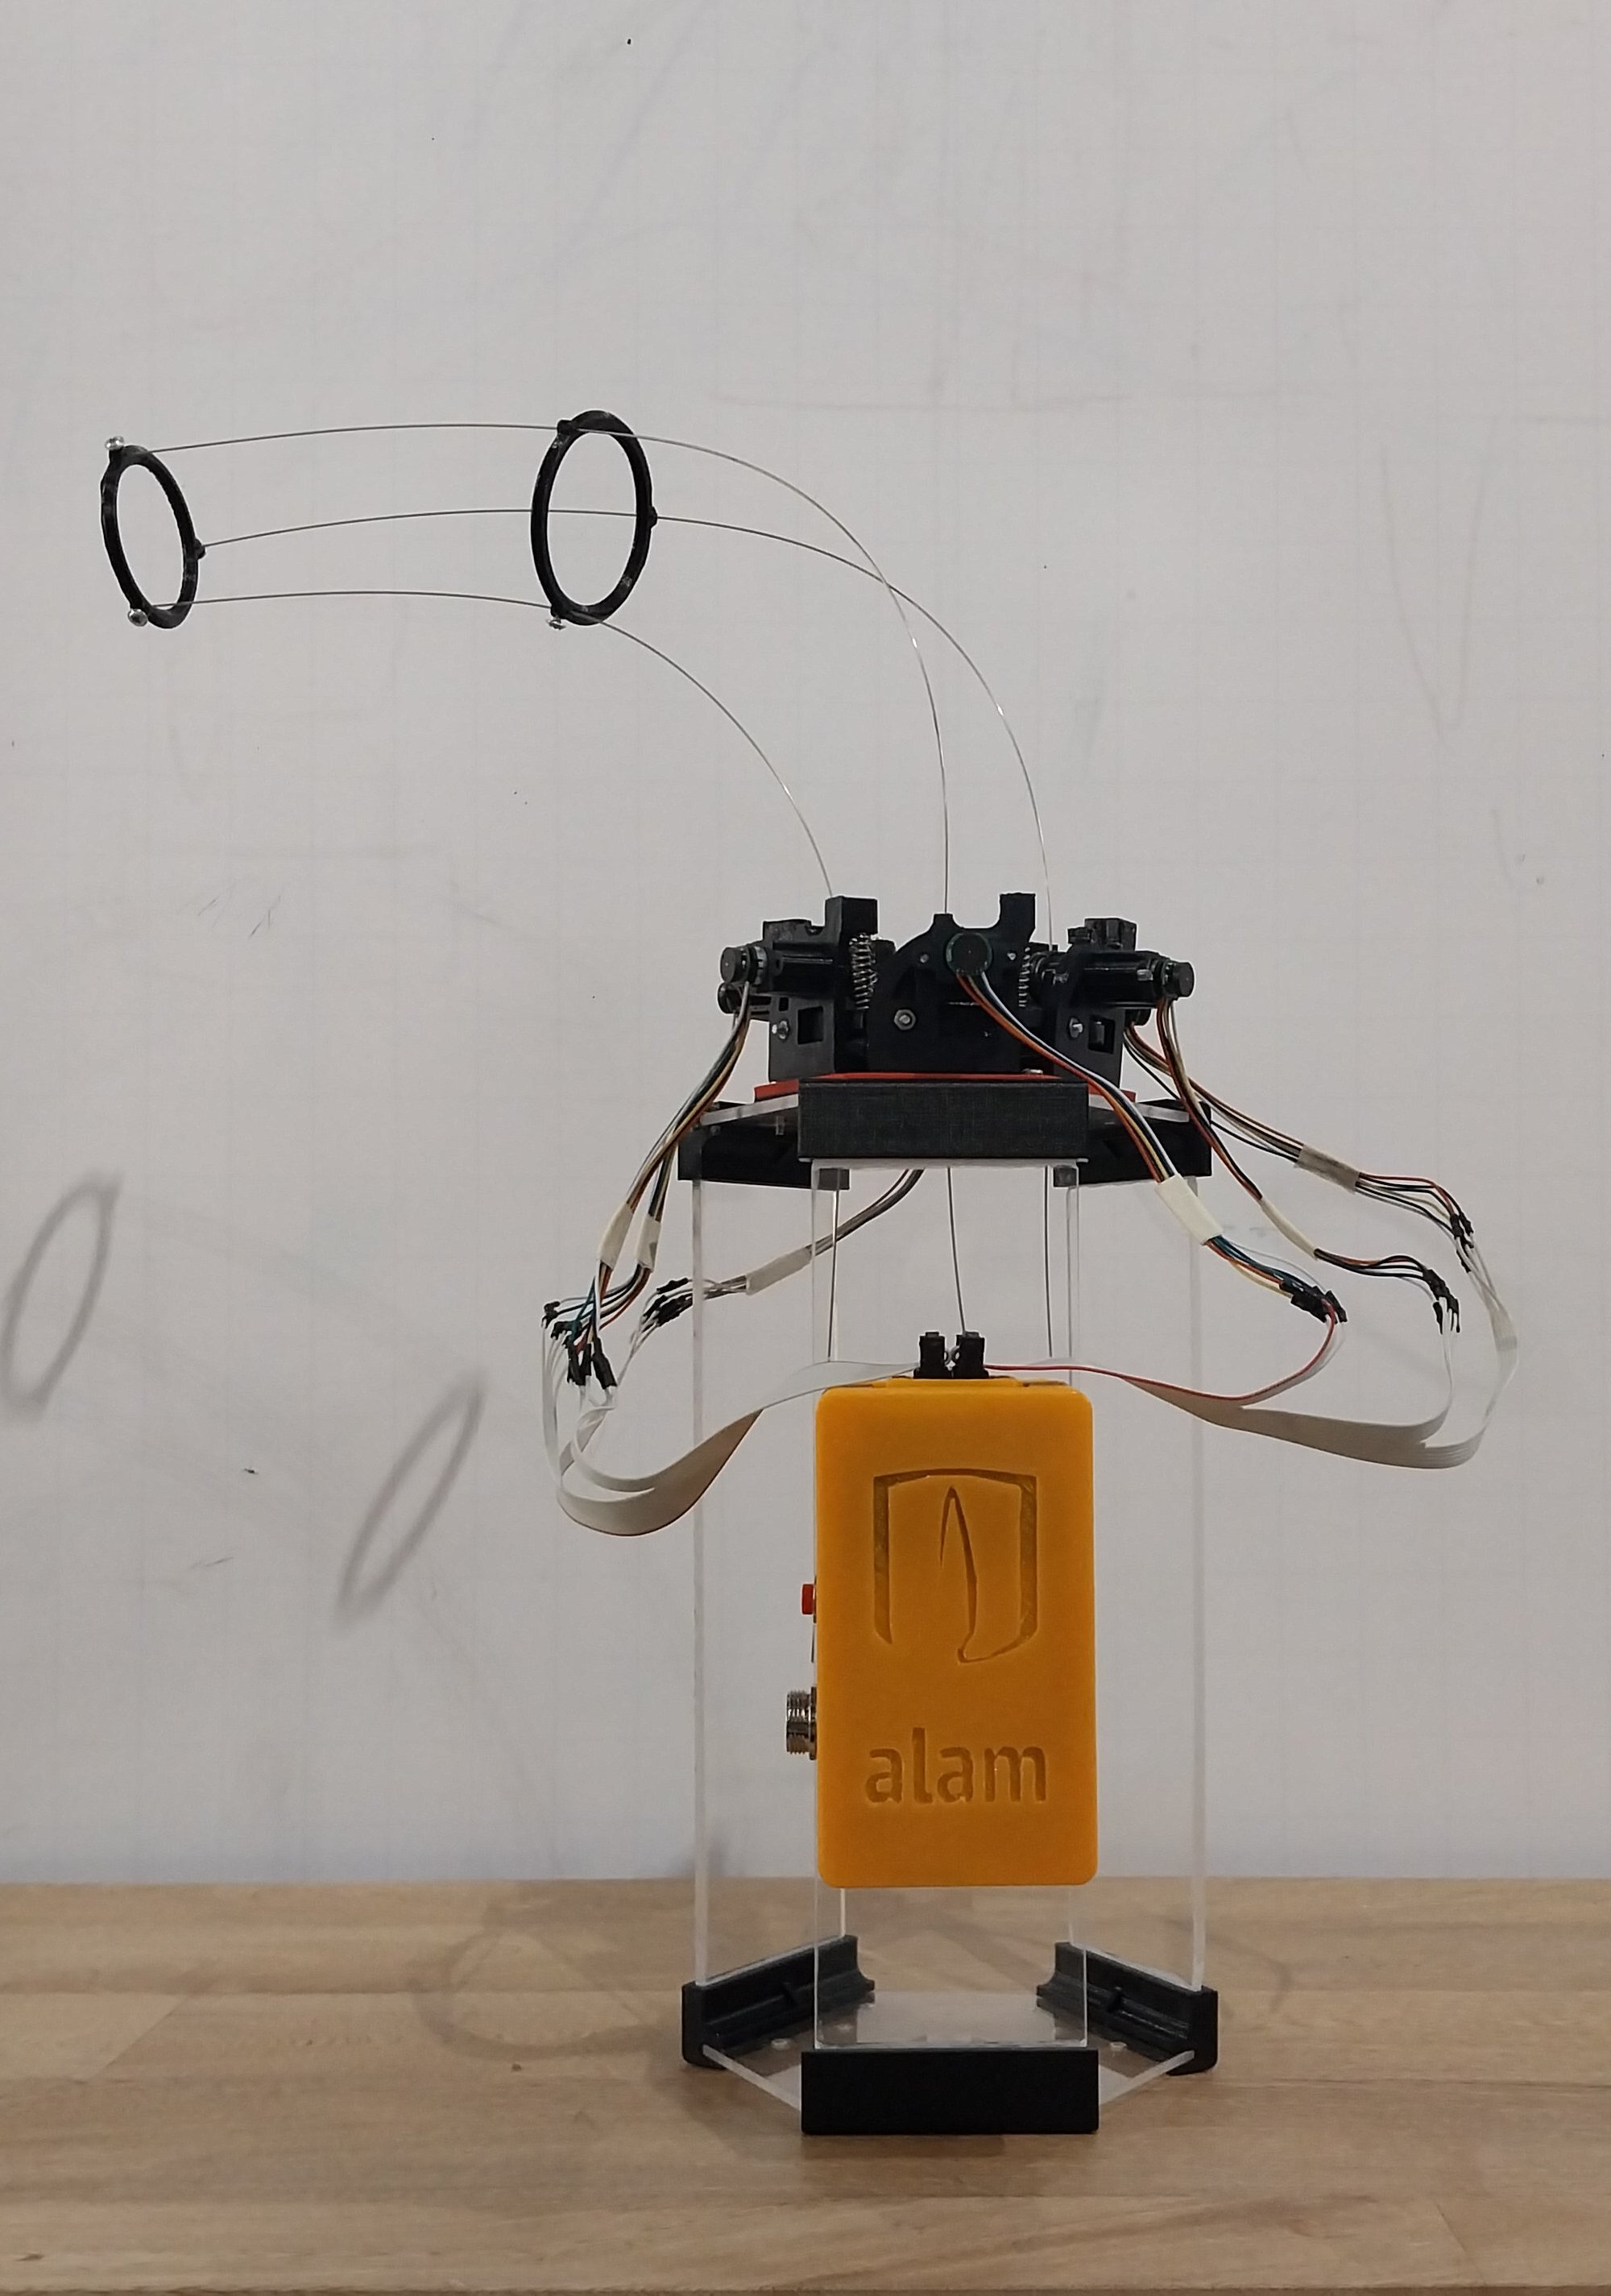
\includegraphics[width=\textwidth]{arm-left}
        \caption{Arm to the left}
        \label{fig:arm-left}
    \end{subfigure}
    \begin{subfigure}[b]{0.3\textwidth}
        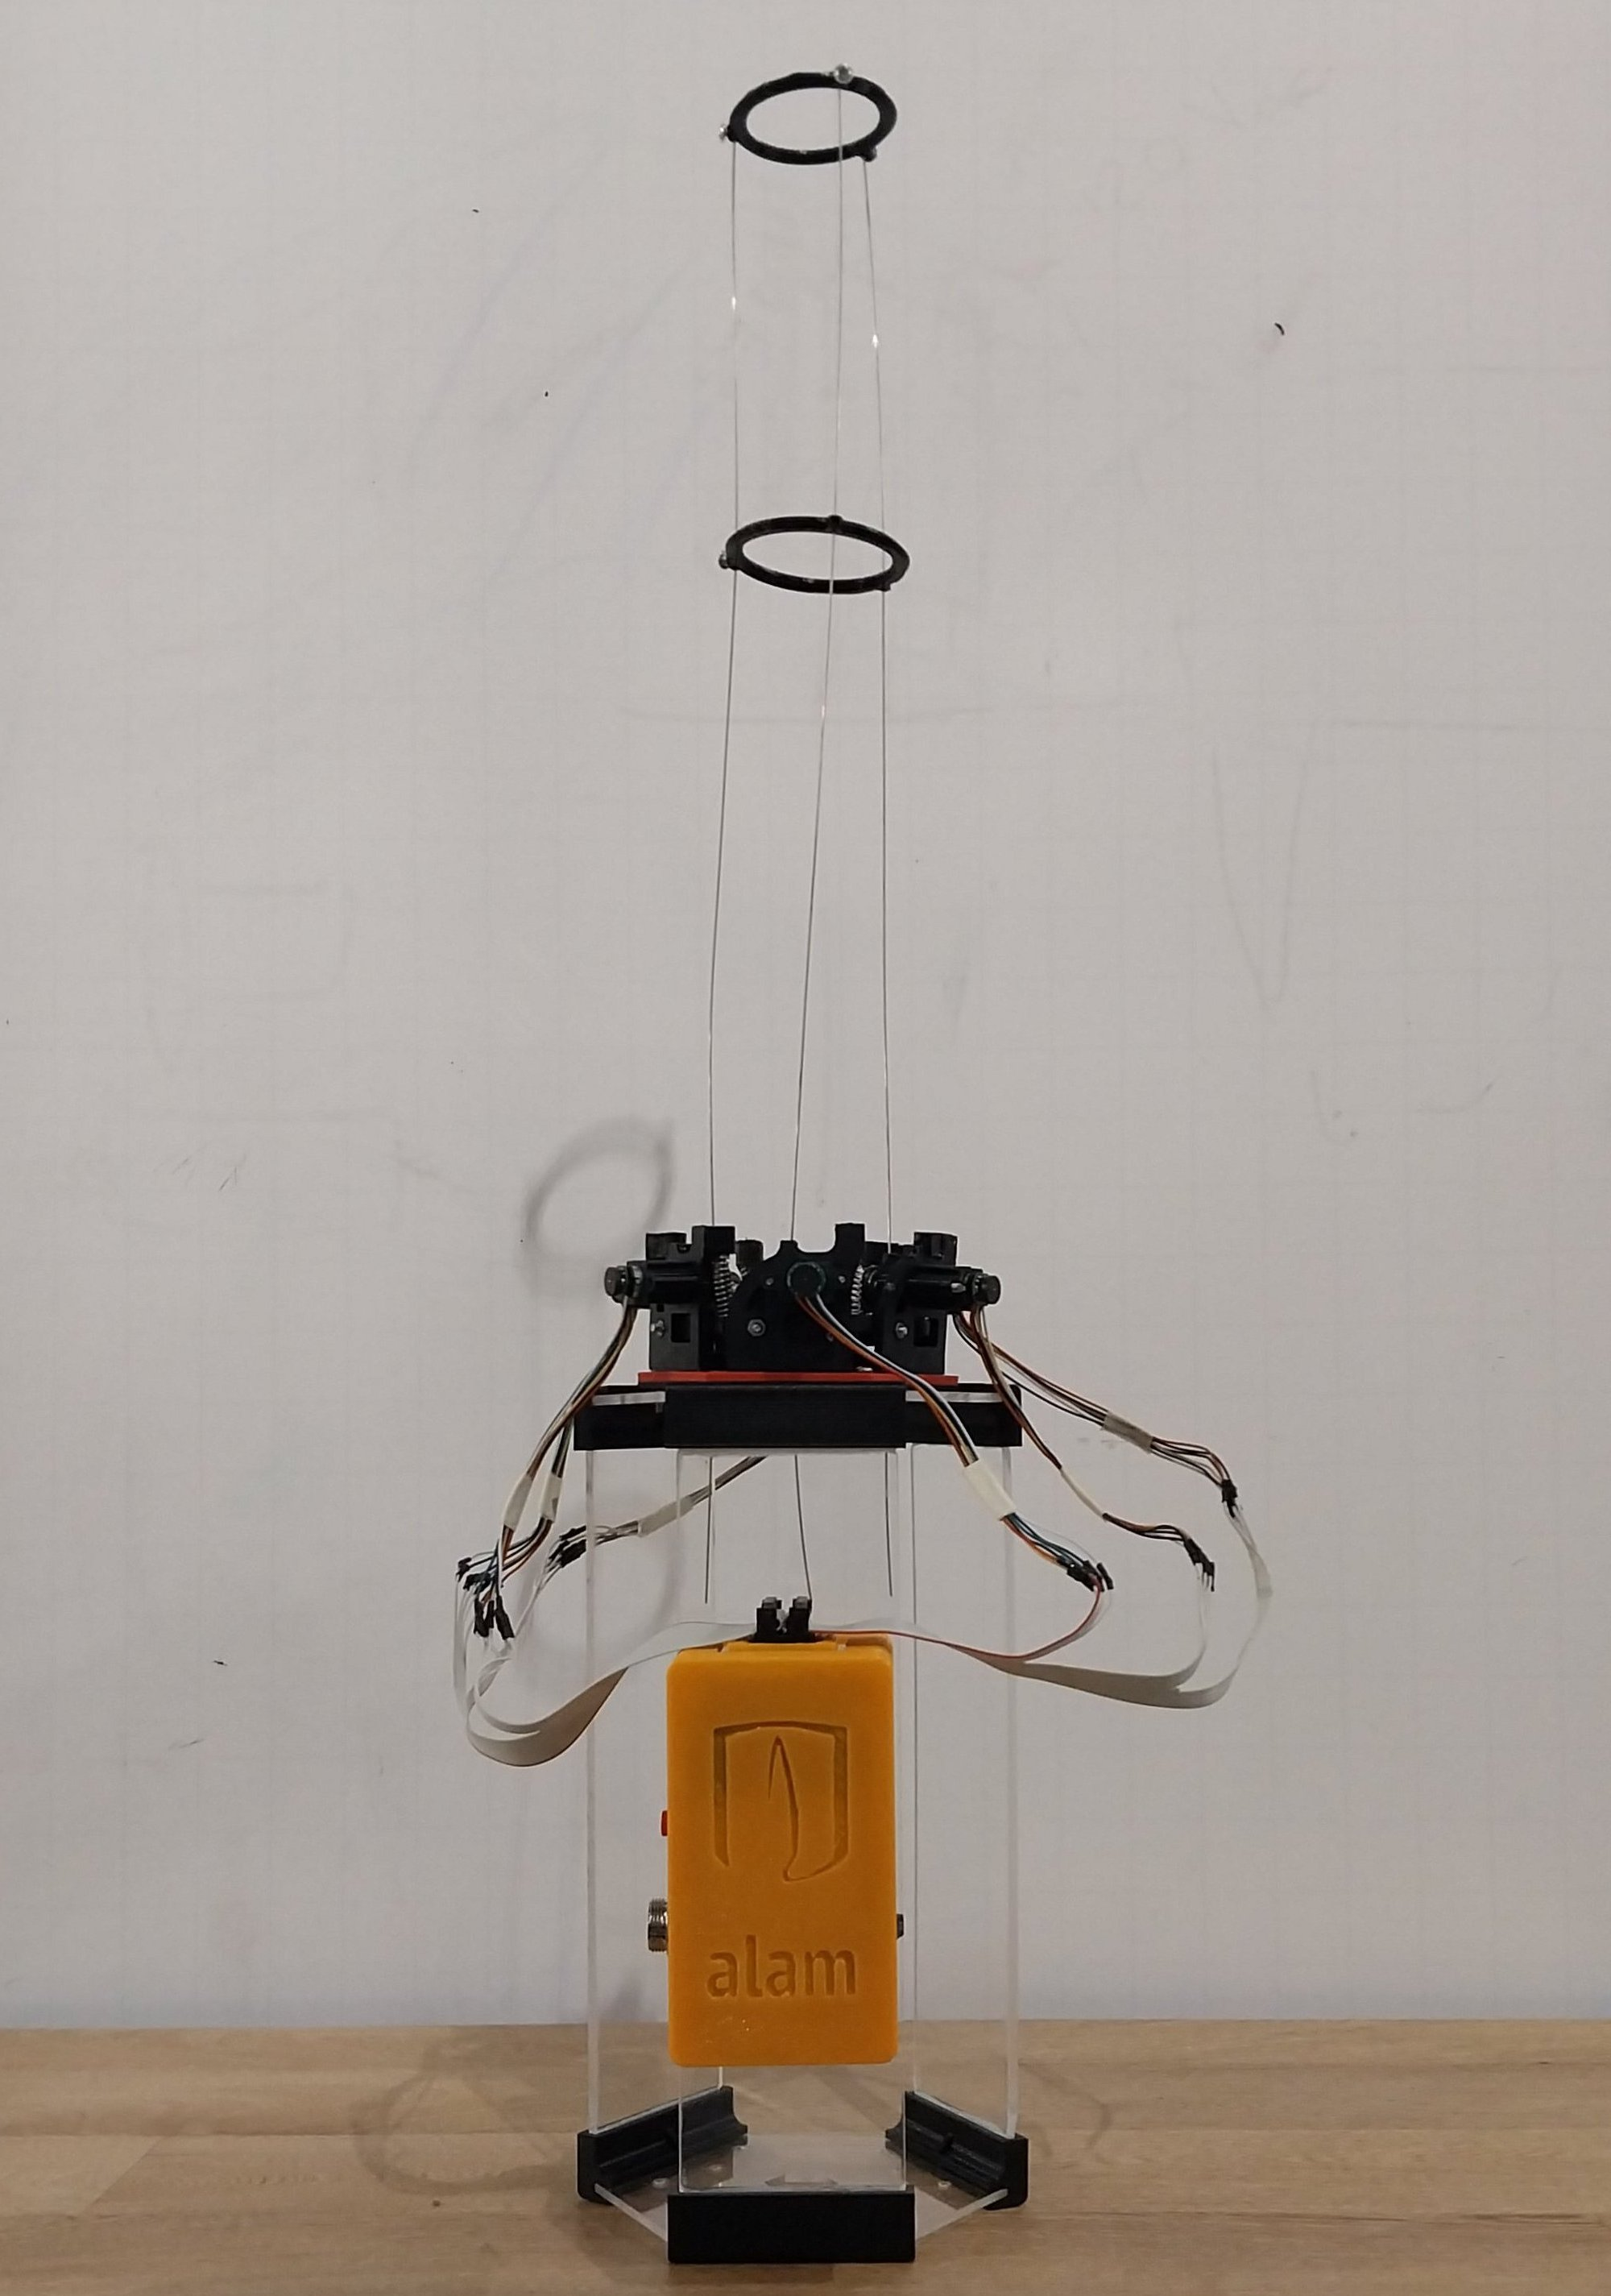
\includegraphics[width=\textwidth]{arm-straight}
        \caption{Straight arm}
        \label{fig:arm-straight}
    \end{subfigure}
    \begin{subfigure}[b]{0.3\textwidth}
        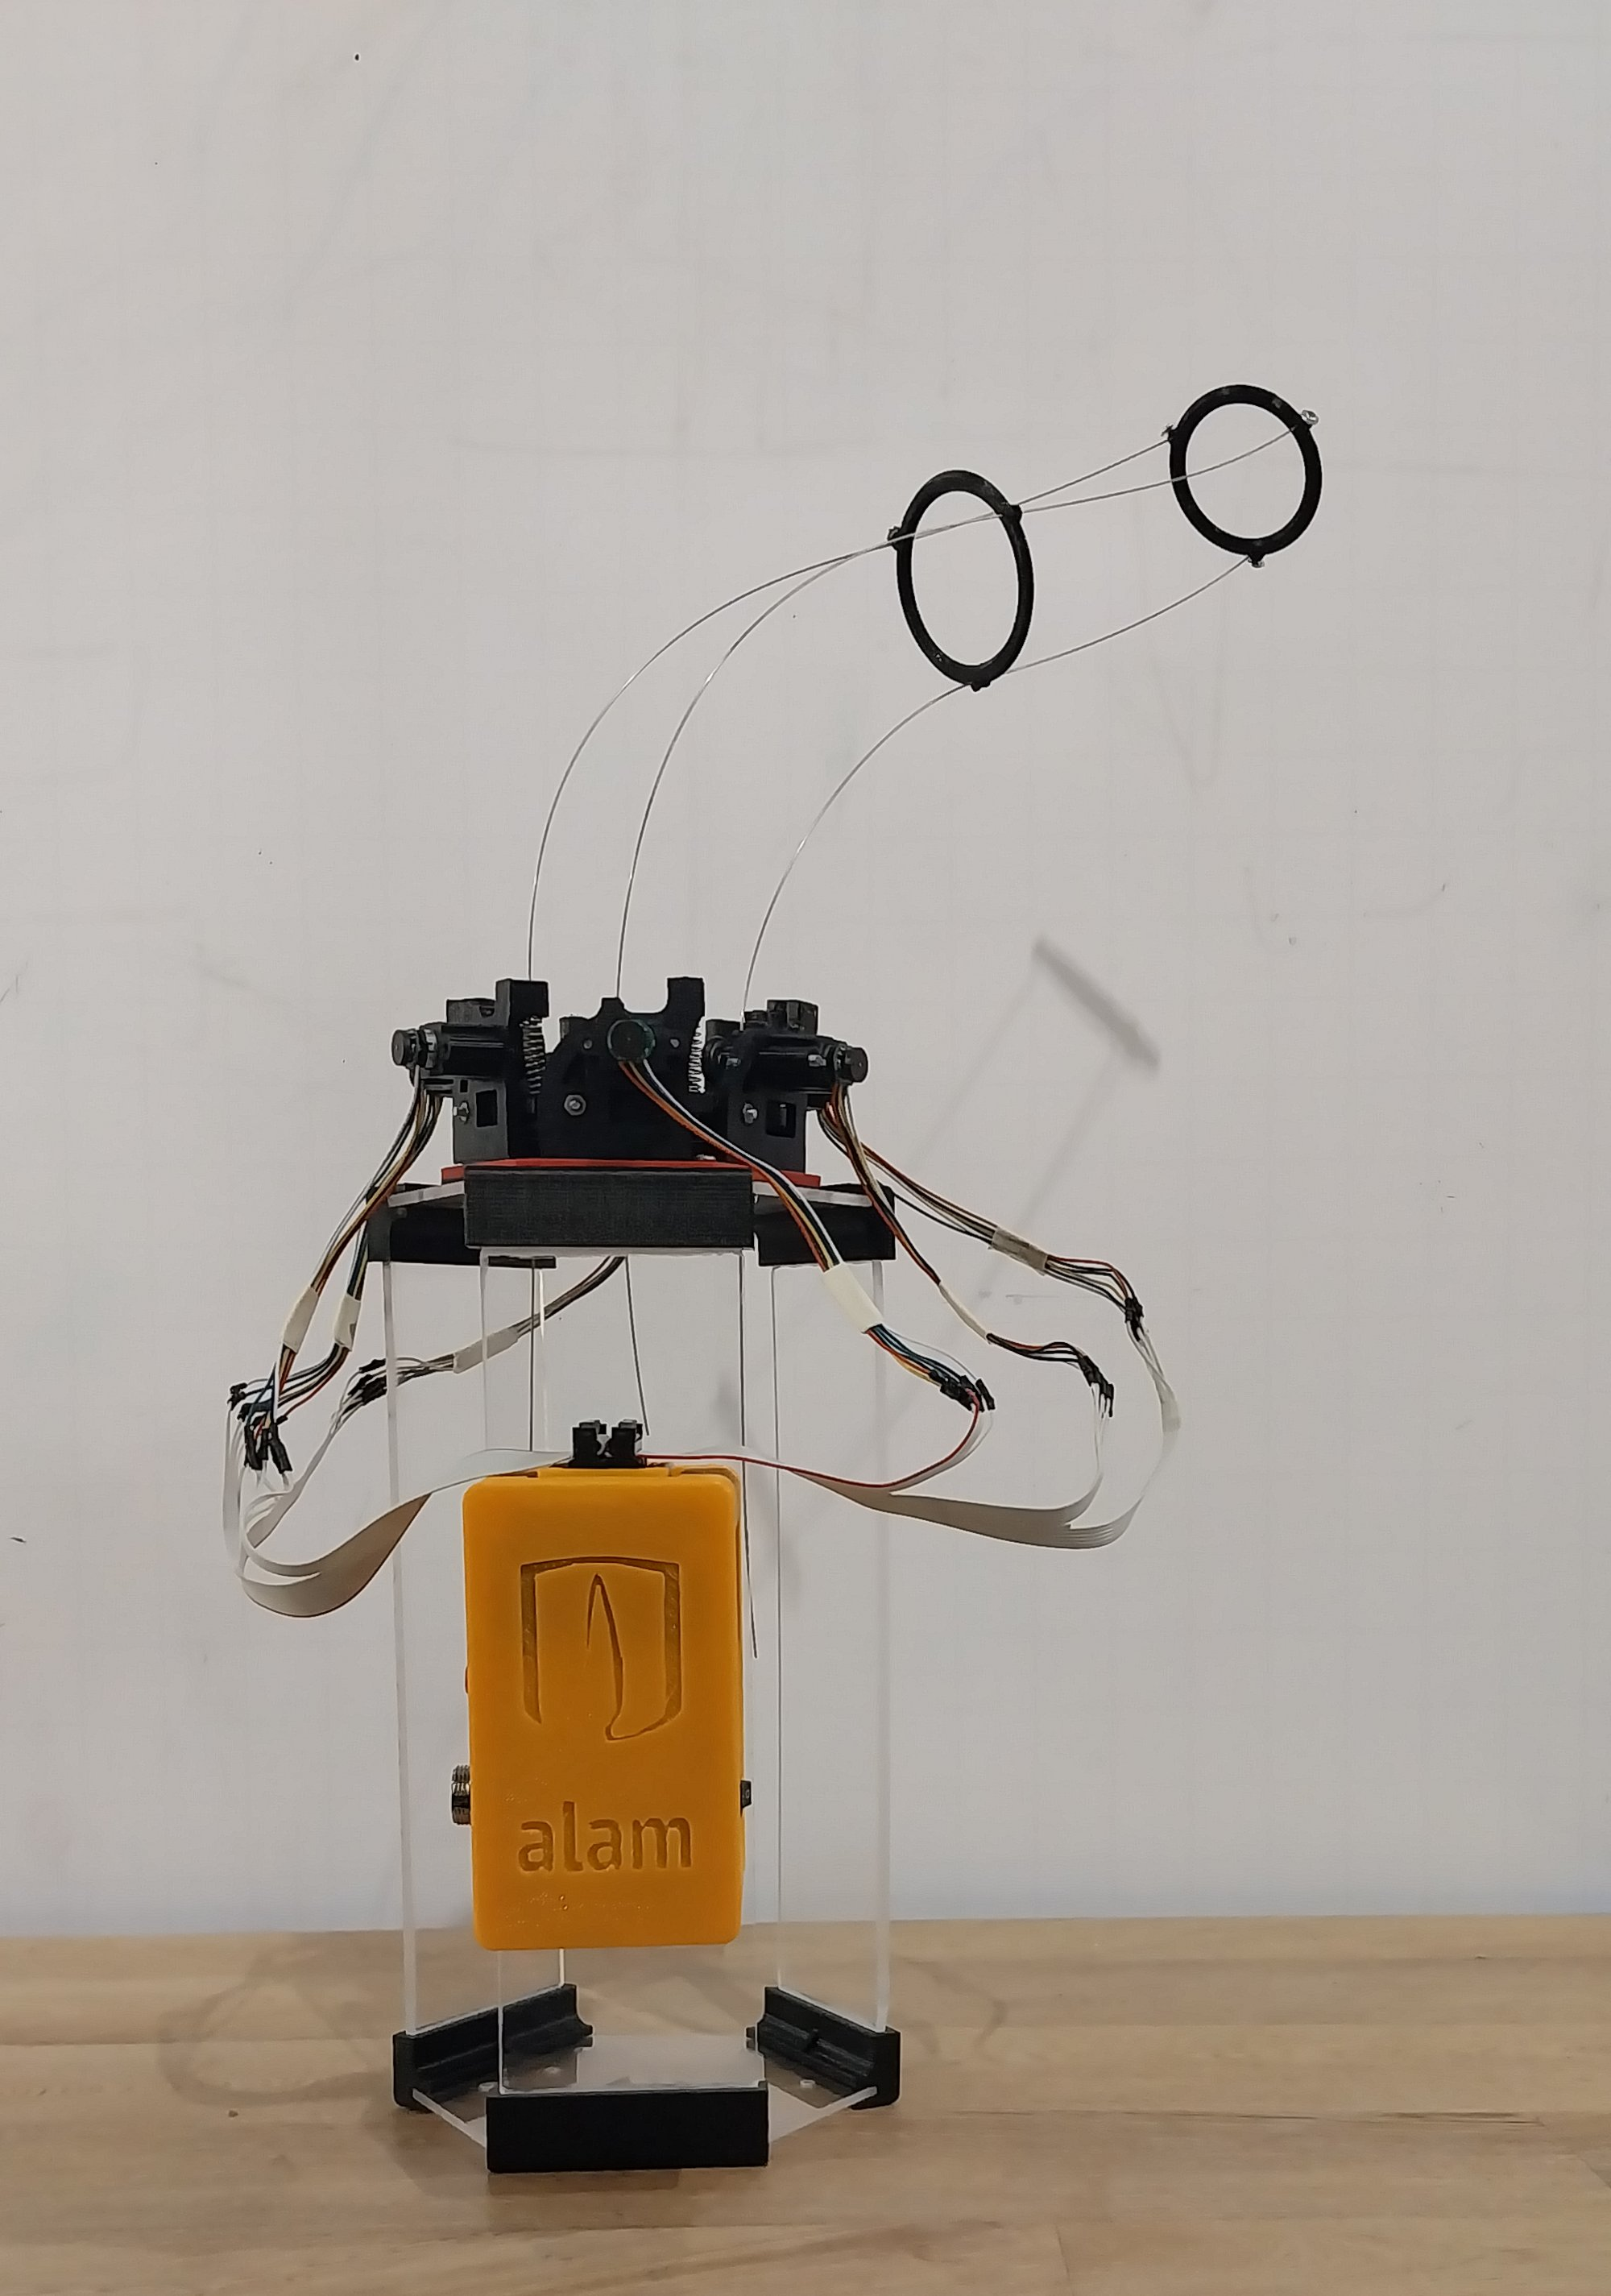
\includegraphics[width=\textwidth]{arm-right}
        \caption{Arm to the right}
        \label{fig:arm-right}
    \end{subfigure}
    \caption{One segment arm positions}
    \label{arm-positions}
\end{figure}

\begin{figure}
    \centering
    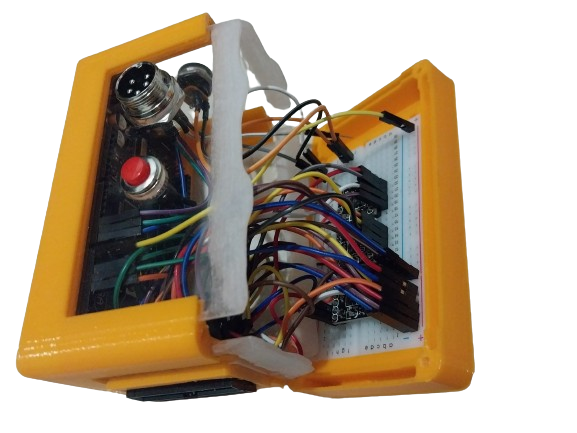
\includegraphics[width=0.6\textwidth]{electronics}
    \caption{Electronics case and connections}
    \label{electronics}
\end{figure}

\begin{figure}
    \centering
    \begin{subfigure}[b]{0.3\textwidth}
        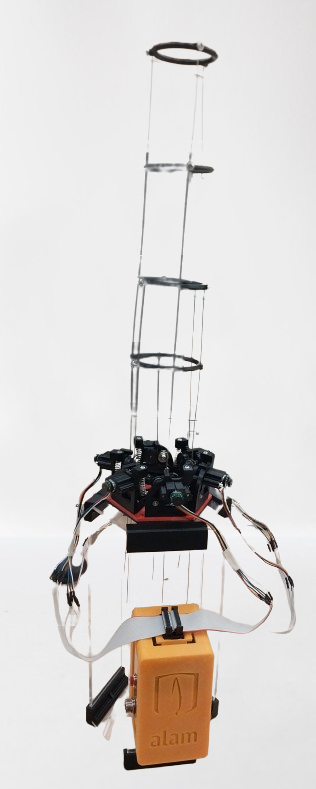
\includegraphics[width=\textwidth]{real-model}
        \caption{Real prototype}
        \label{fig:real-model}
    \end{subfigure}
    \begin{subfigure}[b]{0.3\textwidth}
        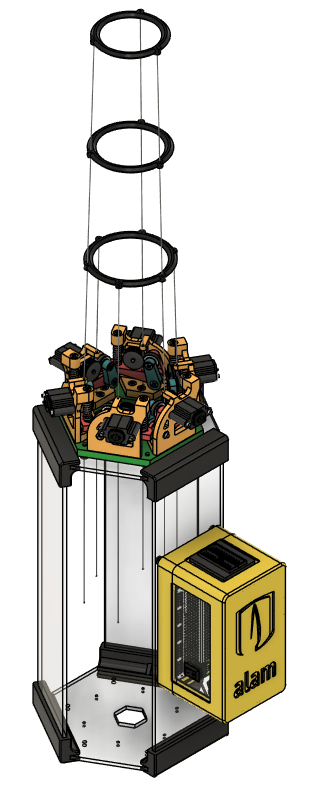
\includegraphics[width=\textwidth]{design-model}
        \caption{Designed prototype}
        \label{fig:design-model}
    \end{subfigure}
    \caption{Complete prototype}
    \label{complete-prototype}
\end{figure}

\begin{figure}
    \centering
    \begin{subfigure}[t]{0.6\textwidth}
        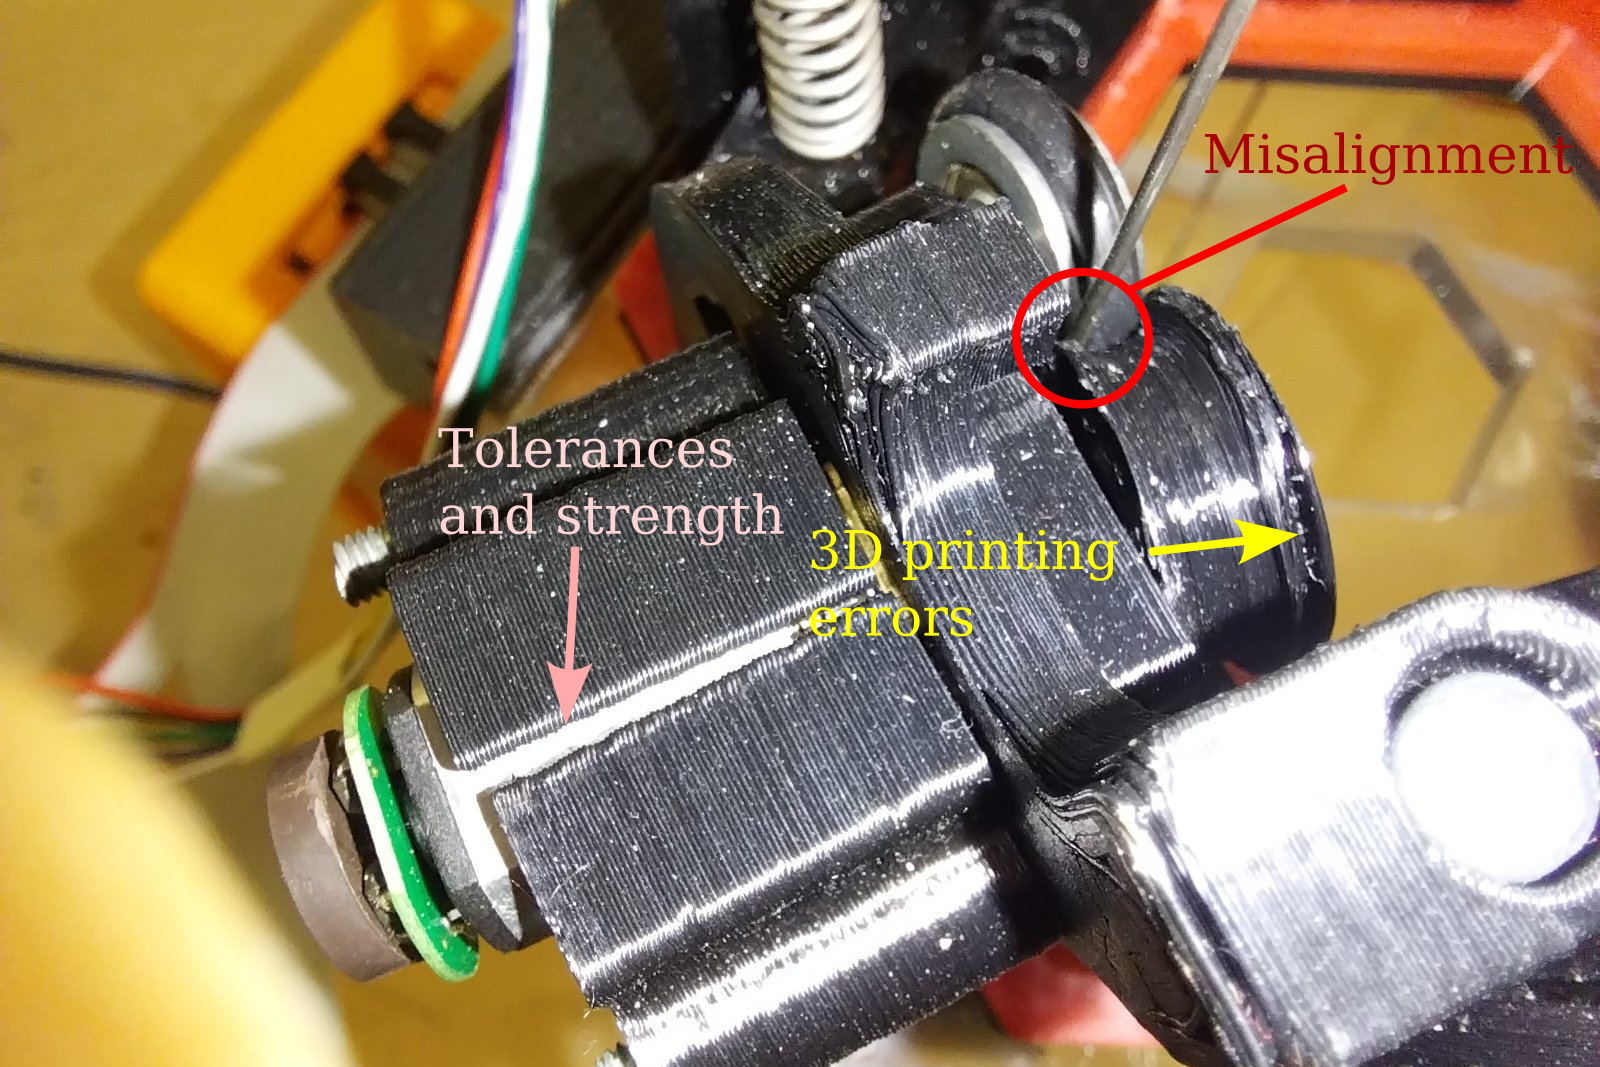
\includegraphics[width=\textwidth]{fdm-issues}
        \caption{Fabrication and alignment}
        \label{fig:fdm-issues}
    \end{subfigure}
    \begin{subfigure}[t]{0.3\textwidth}
        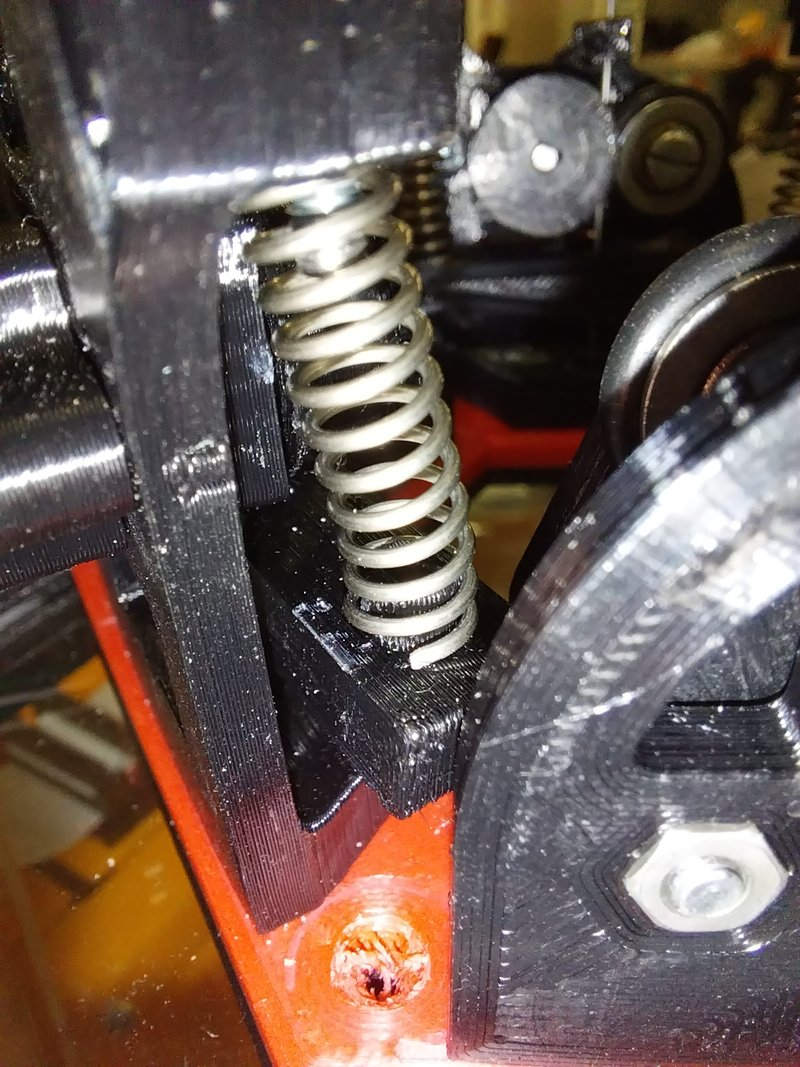
\includegraphics[width=\textwidth]{arm-spring-issue}
        \caption{Spring and arm}
        \label{fig:arm-spring-issue}
    \end{subfigure}
    \caption{Linear actuator issues}
    \label{manufacturing-issues}
\end{figure}


\begin{table}[h]
    \centering
    \caption{Platform specifications}
    \label{tab:platform-specifications}
    \begin{tabular}{ll}
    \toprule
    Property & Value \\
    \midrule
    Height  & 30 cm \\
    Maximum height (with arm) & 70 cm \\
    Weight & 1 kg \\
    Linear actuators tolerance & $\pm$1 mm \\
    \bottomrule
    \end{tabular}
\end{table}